\documentclass{article}
\usepackage[utf8]{inputenc}
\usepackage{amsmath}
\usepackage{amssymb}
\usepackage{amsthm}
\usepackage{enumerate}
\usepackage{mathtools}
\usepackage{float} % For plassering av bilder
\usepackage{a4wide} % mer width
\usepackage{amsmath}
\usepackage{amssymb}
\usepackage{parskip}
\usepackage{xcolor} % Fargelegger matriseelement
\usepackage{verbatim}
\usepackage{makecell} % formatere celler i tabell

\usepackage[colorlinks=false,allcolors=blue]{hyperref}
%Fikser hyperref
\addto\extrasnorsk{%
\def\figureautorefname{Figure}%
\def\tableautorefname{Table}%
\def\sectionautorefname{section}%
\def\subsectionautorefname{subsection}%
}
% Vi endrer fonten som brukes for URLer til den vanlige tekstfonten.
\urlstyle{same}


%Tikz
\usepackage[american]{circuitikz}
\usepackage{tikz}
\usetikzlibrary{patterns}
\usetikzlibrary{arrows.meta}
\usepackage{pgfplots}

% FRA IC
\usepackage{natbib}
\usepackage{amsmath}
\usepackage{listings}
\usepackage{graphicx}

\usepackage[inline]{enumitem}
 \usepackage{booktabs}
\date{}
\newcommand*{\boxednumber}[1]{%
    \expandafter\readdigit\the\numexpr#1\relax\relax
}
\newcommand*{\readdigit}[1]{%
    \ifx\relax#1\else
        \boxeddigit{#1}%
        \expandafter\readdigit
    \fi
}
% Format macro used for every digit, adjust to your liking:
\newcommand*{\boxeddigit}[1]{\fbox{#1}\hspace{-\fboxrule}}

\usepackage[left=4cm,right=4cm,vmargin=1.5cm,footnotesep=0.5cm]{geometry}
\setlength\parindent{0pt}


\title{TDT4265 - Computer Vision and Deep Learning \\Assignment 3}
\author{Jakob Vahlin & Kristian Stensgård}
%\date{September 2020}

\begin{document}

\maketitle

\tableofcontents
\newpage

\section{Task 1: Object Detection Metrics}
\subsection{Task a: Intersection over union}
The intersection over union is a measurement of the overlap between two boundaries. This is used to determine how much of the predicted boundary overlaps with the actual boundary. The measurement is defined as the ratio between the area of the overlap between the two boundaries, and the area of the union over the two boundaries. An illustration of intersection of union is given in \autoref{fig:iou}

\begin{equation}
    \text{IoU} = \frac{\text{Overlap}}{\text{Union}}
\end{equation}

\begin{figure}[H]
    \centering
    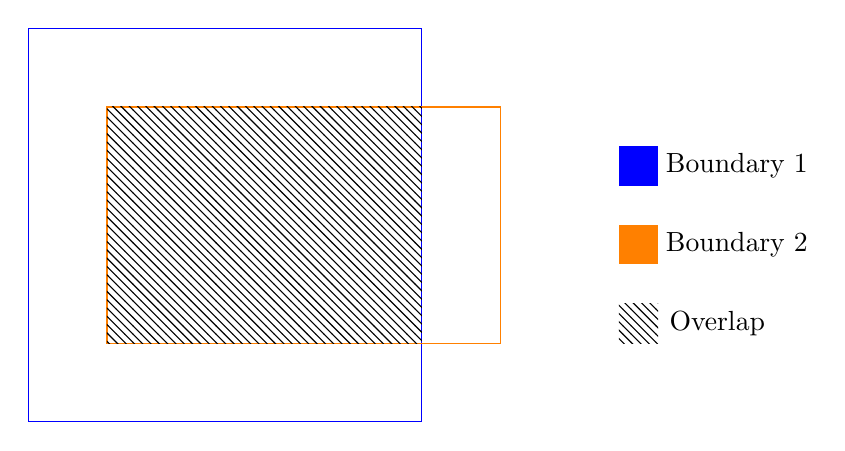
\begin{tikzpicture}
    \draw[blue] (0,0) rectangle (5,5);
    \draw[orange] (1,1) rectangle (6,4);
    \fill [pattern=north west lines] (1,1) rectangle (5,4);
    
    \fill[blue] (7.5,3) rectangle (8,3.5);
    \node at (9,3.25) {Boundary 1};
    
    \fill[orange] (7.5,2) rectangle (8,2.5);
    \node at (9,2.25) {Boundary 2};
    
    \fill[pattern=north west lines] (7.5,1) rectangle (8,1.5);
    \node at (8.75,1.25) {Overlap};
    %\draw [pattern=north west lines] (7.5,1) rectangle (8,1.5);
    
    \end{tikzpicture}
    \caption{An illustration of intersection over union.}

    \label{fig:iou}
\end{figure}


\subsection{Task b: Precision \& Recall}
A \textit{true positive} is a prediction that was predicted as positive, and was correct. \textit{false positive} is a prediction that was predicted as positive, but was not correct.

Precision is a measurement of the accuracy of the predictions. It measures to what extent the predictions were correct. It is defined as the praction between the true positives and the sum of the true and false positives, defined in \autoref{eq:precision}.

\begin{equation}
    \text{Precision} = \frac{\text{Number of True Positives}}{\text{Number of True Positives} + \text{Number of False Positives}}
    \label{eq:precision}
\end{equation}

Recall is a measurement of the extent the model is able to determine the positives. It is defined as the ratio between the True Positive predictions and the sum of the True Positive predictions and False negative predictions, where a \textit{false negative} is a negative prediction that was wrong. Mathematically, recall is defined in \autoref{eq:recall}.

\begin{equation}
    \text{Recall} = \frac{\text{Number of True Positives}}{\text{Number of True Positives} + \text{Number of false positives}}
    \label{eq:recall}
\end{equation}

\subsection{Task c:}

\end{document}